\begin{figure}[tbp]
\centering
\sporkCodeRule
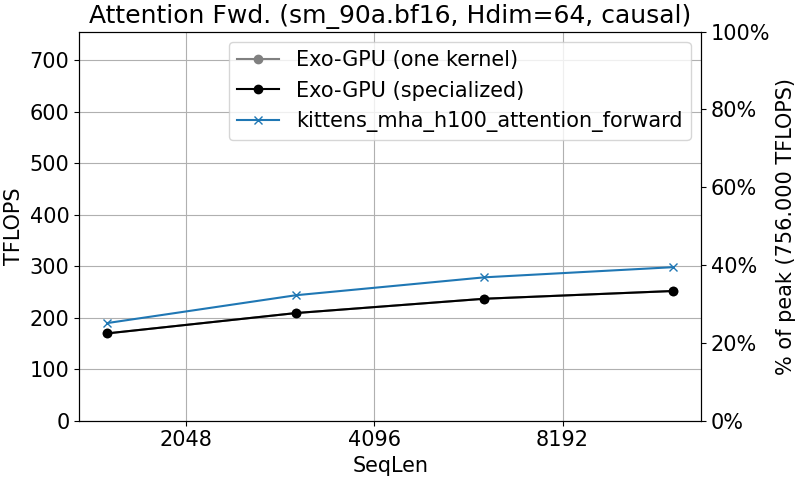
\includegraphics[width=0.45\linewidth]{data-2026-11-11/out_plot/fa/attn_fwd_sm_90a_bf16_h64_causal.png}
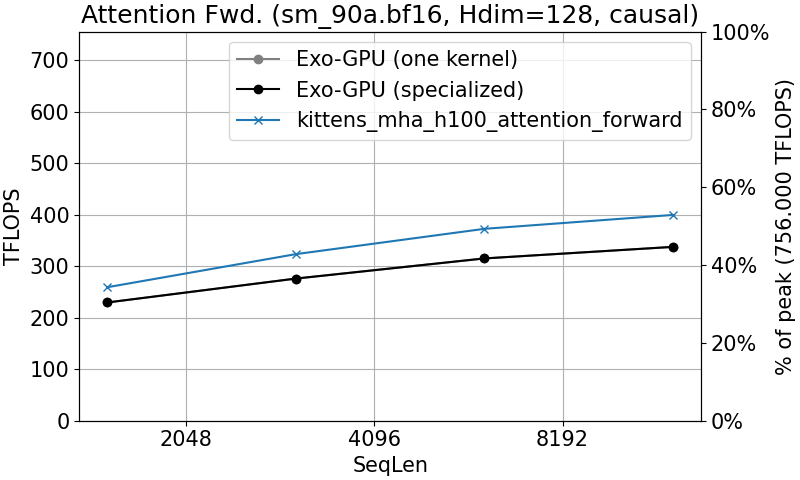
\includegraphics[width=0.45\linewidth]{data-2026-11-11/out_plot/fa/attn_fwd_sm_90a_bf16_h128_causal.png}

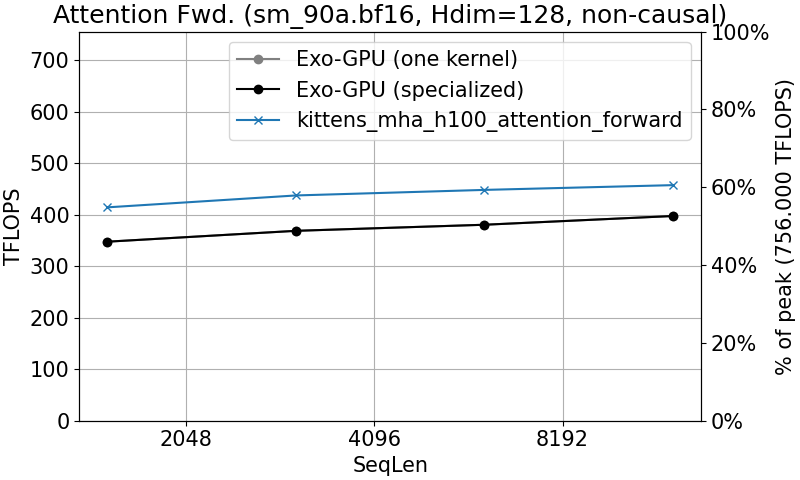
\includegraphics[width=0.45\linewidth]{data-2026-11-11/out_plot/fa/attn_fwd_sm_90a_bf16_h128.png}

\caption{Comparison between \sporkName{} \texttt{sm\_90a} forward attention kernels and ThunderKittens C++,
with bf16 precision.
We estimate that causal attention entails $2 n^2 d$ float ops,
$n$ being sequence length and $d$ being head count times head dimension;
we estimate twice that for non-causal.
}
\label{fig:FaPlots}
\sporkCodeRule
\end{figure}
